%! Author = matt_dumont
%! Date = 14/12/23
%------------------------------------------------------------------
\section[Methods]{Study Methodology}   \label{sec:methods}
%------------------------------------------------------------------
\subsection[Data Processing]{Receptors, Data processing, and analysis} \label{sec:data}

\gls{ecan} provided us with \gls{no3n} concentration data for approximately 100 sites which included groundwater monitoring wells, spring fed streams and the Selwyn Waikirikiri River at Coes Ford.
The Selwyn Waikirikiri River has both hill fed and spring fed components, but in the lower catchment it is a gaining stream and the low flows are dominated by spring fed flow.
We worked collaboratively with \gls{ecan} to select a subset of sites for analysis (\autoref{fig:sitelocs}).
Our final set of sites includes 46 groundwater wells and 10 surface water features.
The raw data and all outputs are available in the \gls{proj_repo} and a summary table of the data is available in \autoref{appx:data}.
Groundwater age data (\gls{mrt} and age distribution parameters) were also provided by \gls{ecan}.
Note that the age data is not available for all sites.

\begin{breakawaybox}[label={box:mrt}]{How mean residence time is identified}
    Groundwater ages are typically estimated from measured environmental tracers such as \gls{cfc}, \gls{h3} and \gls{sf6}.
    We have historical atmospheric concentrations of these tracers and, because these tracer are conservative (concentrations do not change over time) or breakdown in a constant rate can use them to estimate the age of the groundwater. This is typically done using simple 1d mixing models, such as the \gls{epfm}. These mixing models provide a distribution of ages for the water in the sample and the mean of this distribution is the \gls{mrt}. Because these mixing models simplify the systems there is some inherent, often unquantified, uncertainty in the age estimates. Nevertheless, these ages provide useful constraints on the distribution of ages in the aquifer and are useful for understanding the potential pathways of contaminants.

\end{breakawaybox}

The data was processed as follows:
\begin{enumerate}
    \item \textbf{Outlier Identification}: we identified two types of outliers (see \autoref{fig:ex_outlier_trend}):
    \begin{enumerate}
        \item  True outliers: values which based on a statistical and visual analysis were clearly outside the measured values for the site. These values were removed from the dataset. It is worth noting that these \say{true outliers} are not necessarily erroneous data, but they are not representative of the site's typical \gls{no3n} concentration. For instance, recharge events can cause a spike in \gls{no3n} concentration, which is not representative of the long-term trend.
        \item Trend outliers: data which precede the most recent / current trend and could erroneously affect the fit of the current historical trend. These values were not included in the historical trend analysis or \gls{no3n} noise estimation.
    \end{enumerate}
    \item \textbf{Estimate the age distribution, wells}: where sites did not have age sampling and modelled groundwater age distributions we estimate the parameters from nearby sites. The method was somewhat manual and was often site specific. Details on how we estimated the age distribution for each site are available in the \gls{proj_repo}.
    \item \textbf{Estimate the age distribution, streams}: There was no age estimates for the spring fed streams and the Selwyn-Waikirikiri; therefore we assessed the detection power assuming a range \gls{mrt} values: 5, 10, 20, and 30 years. The other age model parameters were assumed to be the median of all sites within (7.5 or 10 km) and <=10m depth. Further details are available in the \gls{proj_repo}
\end{enumerate}

\kslfig {0.90\textwidth}{figures/m36_8187}{Site M36/8187: note the "true" outliers (black) and the trend outliers(red)}{ex_outlier_trend}{}

\begin{landscape}
    \kslfig{1.25\textheight}{../figures/selwyn_sites}{Final Site Locations}{sitelocs}{}
\end{landscape}


%------------------------------------------------------------------
\subsection[Pathways]{Assumed Pathways} \label{subsec:apriori}

In consultation with \gls{ecan} we generated the following \textit{a. priori} pathways for the implementation of \gls{no3n} reductions:
\begin{itemize}
    \item \textbf{No change}: no change in \gls{no3n} source concentrations.
    \item \textbf{5\% reduction}: a 5\% reduction in \gls{no3n} source concentrations implemented linearly between 2017 and 2022.
    \item \textbf{10\% reduction}: a 10\% reduction in \gls{no3n} source concentrations implemented linearly between 2017 and 2022.
    \item \textbf{20\% reduction}: a 20\% reduction in \gls{no3n} source concentrations implemented linearly between 2017 and 2022.
    \item \textbf{30\% reduction}: a 30\% reduction in \gls{no3n} source concentrations implemented linearly between 2017 and 2022.
\end{itemize}

While \gls{pc1} specifies the required nitrate load reductions, it does not apply to all land uses.
The source zones for wells and spring fed streams will comprise a mixture of land use types and hence nitrate load loss reduction rates, but these source zones are either unknown or poorly constrained.
the mandated nitrate reduction rate within the catchment area of each monitoring site could range between zero (if the catchment/source zone encompasses only land uses for which nitrate load loss reductions are not required) and 20\% (if the catchment contains only high intensity land use for which a 20\% reduction is required).
We therefore modelled a range of nitrate loss reductions (aka assumed pathways).
A higher-than-expected reduction pathway (30\%) was also included to explore the potential impact of better than expected nitrate loss reductions on change detection monitoring.

%------------------------------------------------------------------
\subsection[Detection Power Methods] {Detection Power Methods} \label{subsec:detection_power_methods}

The method to calculate the detection power of a given site was implemented after \citet{dumont_determining_nodate}
using our open source package\citep{dumont_komanawagw_detect_power_2023}.
Briefly the methodology is as follows for each site:

\begin{wrapfigure}{R}{0.70\textwidth}
    \begin{breakawaybox}[label={box:dp}]{What is Detection Power}
        Detection power is the percent probability of detecting a statistically robust trend in the receptor concentration time series. Noisy data reduces the detection power while more frequent sampling increases the detection power.
        \\
        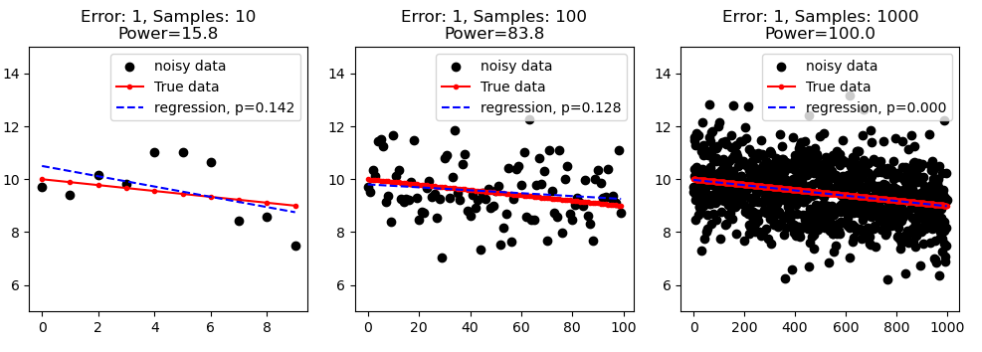
\includegraphics[width=0.95\textwidth]{figures/dp_ex}
    \end{breakawaybox}
\end{wrapfigure}

\begin{enumerate}
    \item Ascertain whether the historical concentration data has a statistically robust trend (e.g. via a Mann-Kendall test, see \autoref{fig:ex_outlier_trend})
    \item Estimate the noise in the receptor concentration time series
    \begin{enumerate}
        \item If the historical concentration data has an increasing statistically robust trend, then the noise can be estimated as the standard deviation of the residuals from a model (e.g. a linear regression or Sen-slope/ Sen-intercept).
        \item If the historical concentration data does not have a statistically robust trend, then the noise can be estimated as the standard deviation of the receptor concentration time series.
        \item If the historical concentration data has a statistically robust decreasing trend, we assumed that the receptor was at steady state and considered the site in the same fashion as a site with no statistically robust trend. This assumption was used because it is very difficult to estimate the historical pathway of a decreasing trend as the maximum concentration is unconstrained. While this will likely underestimate the detection power, it is a conservative approach and only affects a small number of sites (only 3 of 46 sites in this study).
    \end{enumerate}
    \item Estimate the average source zone concentration (i.e., at the base of the root zone) from the historical trend (if any) and the groundwater age distribution.
    \item Predict the true receptor concentration time series (e.g., the concentration at the receptor if there was no noise) based on the aforementioned source concentration, assumed pathway and the groundwater age distribution.
    \item Resample the true receptor concentration time series to the desired sampling frequency and duration (e.g., quarterly sampling for 10 years).
    \item Calculate the statistical probability of detecting the change
    \begin{enumerate}
        \item generate a synthetic sample of the receptor noise (e.g., by sampling a normal distribution)
        \item add the synthetic noise to the true receptor concentration time series
        \item conduct a statistical test (here we used a Mann-Kendall test or a Multipart Mann Kendall test) to determine if the synthetic receptor concentration time series has a statistically robust trend
        \item repeat steps a-c many times (we used 1000 iterations). The probability of detecting the change is the number of times the synthetic receptor concentration time series had a statistically robust trend divided by the number of iterations.
    \end{enumerate}
\end{enumerate}

The source concentration was estimated by fitting a simple source to receptor model.
The source concentration was set via a parameterised trend and minimum value.
The assumption is that the source concentration has been monotonically increasing with time from a minimum value of 0.01 mg/l \gls{no3n}.
The source concentration was then transformed to the receptor concentration via the \gls{epfm}.
We then conducted curve fitting to find the best fit of the source concentration to the receptor concentration.
\autoref{fig:source_ex} provides an example of the source concentration estimation.
Site M36/0698 has a statistically robust increasing trend, approximately 0.12 mg/l/yr \gls{no3n}.
Given the \gls{mrt} of 22.75 years the best fit of the data (solid gold line) suggests that the peak source concentration is likely to be c. 7 mg/l \gls{no3n} (dashed gold line).
More details on this process are available in \citet{dumont_determining_nodate, dumont_komanawagw_age_tools_2023}

\kslfig {.95\textwidth}{figures/m36_0698_red20_true_conc}{Site M36/0698 as an example of the source concentration prediction}{source_ex}{}

For the statistical test we used:
\begin{itemize}
    \item A \textbf{Mann-Kendall test} for sites without an increasing trend
    \item A \textbf{Multipart Mann-Kendall test} for sites with an increasing trend. We used a Multipart Mann-Kendall test here as an increasing trend can continue after the implementation of \gls{pc1}, due to historical increases in \gls{no3n} source concentrations which have not reached steady state at the receptor. A traditional Mann-Kendall test would require the absolute knowledge of the time of the maximum \gls{no3n} receptor concentration. A Multipart Mann-Kendall test does not require this knowledge. For more information see \citet{dumont_komanawakendall_stats_2023}
\end{itemize}

We set the critical level at 5\% (<0.05) for both tests.
For the Mann-Kendall test this means that the trend was detected if p<0.05. For the multipart Mann-Kendall test this means that the trend was detected if there was any breakpoint where the older data was increasing (p<0.05) and the newer data was decreasing (p<0.05).
Note that a minium of 5 datapoints were required for each part in the multipart Mann-Kendall test.
Finally, some sites will not have a decreasing \gls{no3n} concentration because the implemented nitrate loss reduction is insufficient to reduce steady state concentrations below the current level.
In this case the aforementioned multipart Mann-Kendall test would never detect a trend.
Therefore, we conducted a subsequent multipart Mann-Kendall test which identified a breakpoint where there was an earlier increasing trend (p<0.05) and subsequently no trend (p>0.5). These plateau sites are further discussed in \autoref{sec:plateau_results}.

\begin{breakawaybox}[label={box:mrttoconc}]{Source to Receptor Concentration}
    The receptor concentration at a given time is calculated from the source concentration using a \gls{epfm}.
    For instance below the concentration in the receptor at 2014-10-21 (red circle) is calculated as the sum of the source concentration time series times (plot 1) the proportion of the water in the receptor on 2014-10-21 that originated from the source at that time (plot 2).
    \\
    \begin{center}
        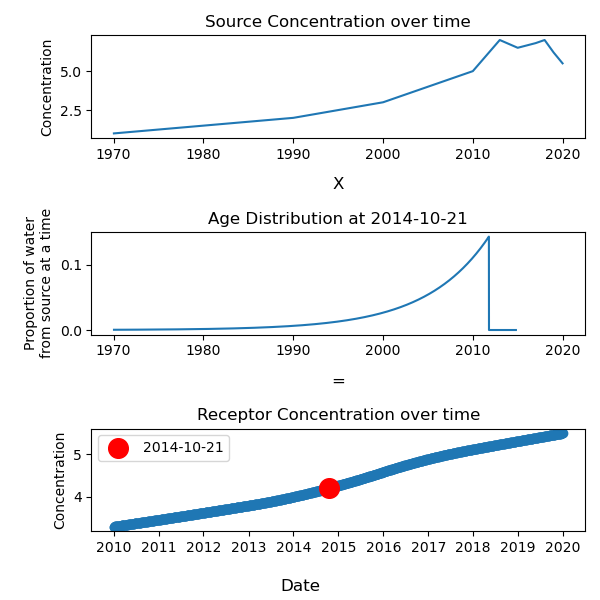
\includegraphics[width=0.65\textwidth]{../GeneratedData/mrt_explain_fig}
    \end{center}
\end{breakawaybox}